\subsection{Liver CT Feedback: Preliminary Results}
We trained a Na\"{i}ve Bayes classifier to predict the diagnosis of liver lesions given radiologist descriptors. We then implemented a greedy feature selection algorithm to minimize expected entropy of class distribution. This feedback method was compared to random feature selection as a baseline feedback method. We see qualitatively that the performance of the minimum entropy feature selection converges to maximum classification accuracy in much fewer features than random selection (Figure \ref{fig:liver_feedback}). Our next step here is to add a stopping criteria (e.g. threshold on distribution entropy) to measure the expected accuracy of such a system.

\begin{figure}[h]
\centering
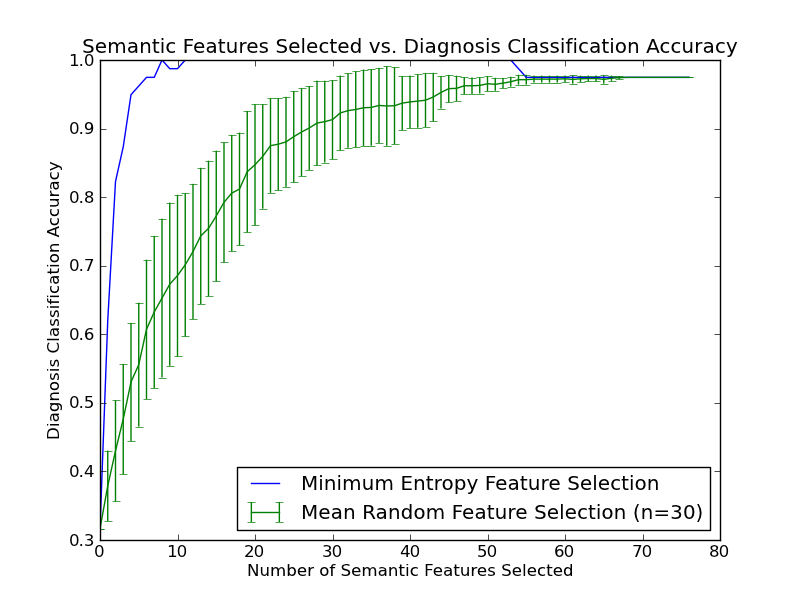
\includegraphics[width=\linewidth]{liver_feedback.png}
\caption{Comparison of mutual information to random selection criteria in diagnosis of liver lesions}
\label{fig:liver_feedback}
\end{figure}


\clearpage
\subsection{Mammography Feedback: Preliminary Results}
We trained a Tree-Augmented Na\"{i}ve Bayes classifier to predict the diagnosis of malignancy in mammography reports. We then tested two feedback methods over 20 possible BI-RADS descriptors. Once again, we compared this to random feature selection, and did not use any stopping criteria. Figure \ref{fig:feedback_mammo} shows the results of the feedback methods. Notably, minimizing expected entropy was equivalent to maximizing mutual information. Furthermore, we measured the feature ranks using mutual information. This was the mean rank of each feature selected, so lower valued ranks are considered most important.

\begin{figure}[h]
	\centering
	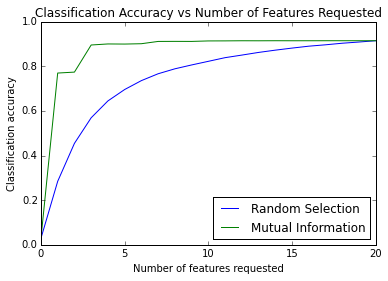
\includegraphics[width=\linewidth]{feedback_mammo.png}
	\caption{Comparison of mutual information to random selection criteria in diagnosis of mammography lesions}
	\label{fig:feedback_mammo}
\end{figure}


\begin{figure}[h]
	\centering
	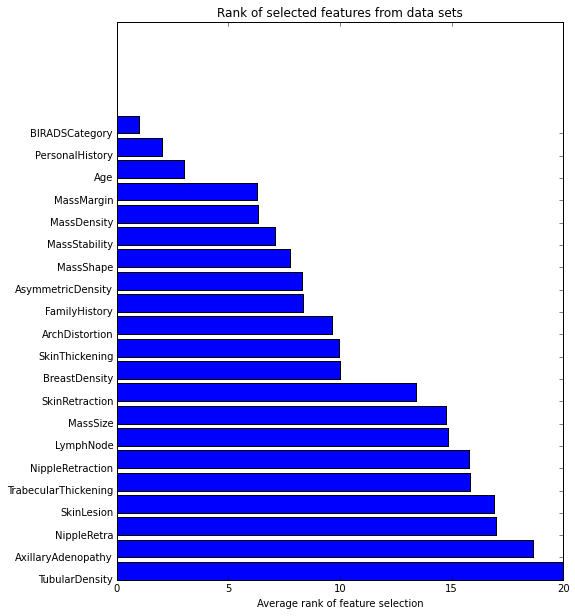
\includegraphics[width=\linewidth]{feedback_mammo_ranks.png}
	\caption{The selection rank of different features in mammography reports. Lower values mean more important}
	\label{fig:feedback_mammo_ranks}
\end{figure}